%===== Chapter 3: System Design and Architecture =====%

\chapter{System Design and Architecture}

\section*{Introduction}
This chapter translates the requirements into a concrete system design, covering
the global architecture, database schema, API structure, and key interaction flows.

\section{Global Architecture}

\subsection{Three-Service Architecture}

Malltech is decomposed into three independently deployable TypeScript services:

\begin{longtable}{|m{4cm}|m{2.5cm}|m{7cm}|}
    \hline
    \textbf{Service}           & \textbf{Framework} & \textbf{Role}                                           \\
    \hline
    \endhead
    \endfoot
    \endlastfoot
    \hline
    \texttt{malltech-backend}  & NestJS 11          & RESTful API, business logic, WebSocket gateway, MongoDB \\
    \hline
    \texttt{malltech-frontend} & Next.js 16         & Customer storefront (SSR/SSG)                           \\
    \hline
    \texttt{malltech-admin}    & Next.js 16         & Administration backoffice dashboard                     \\
    \hline
    \caption{Malltech service decomposition}
    \label{tab:services}
\end{longtable}

\subsection{Deployment Architecture}

\begin{figure}[H]
    \centering
    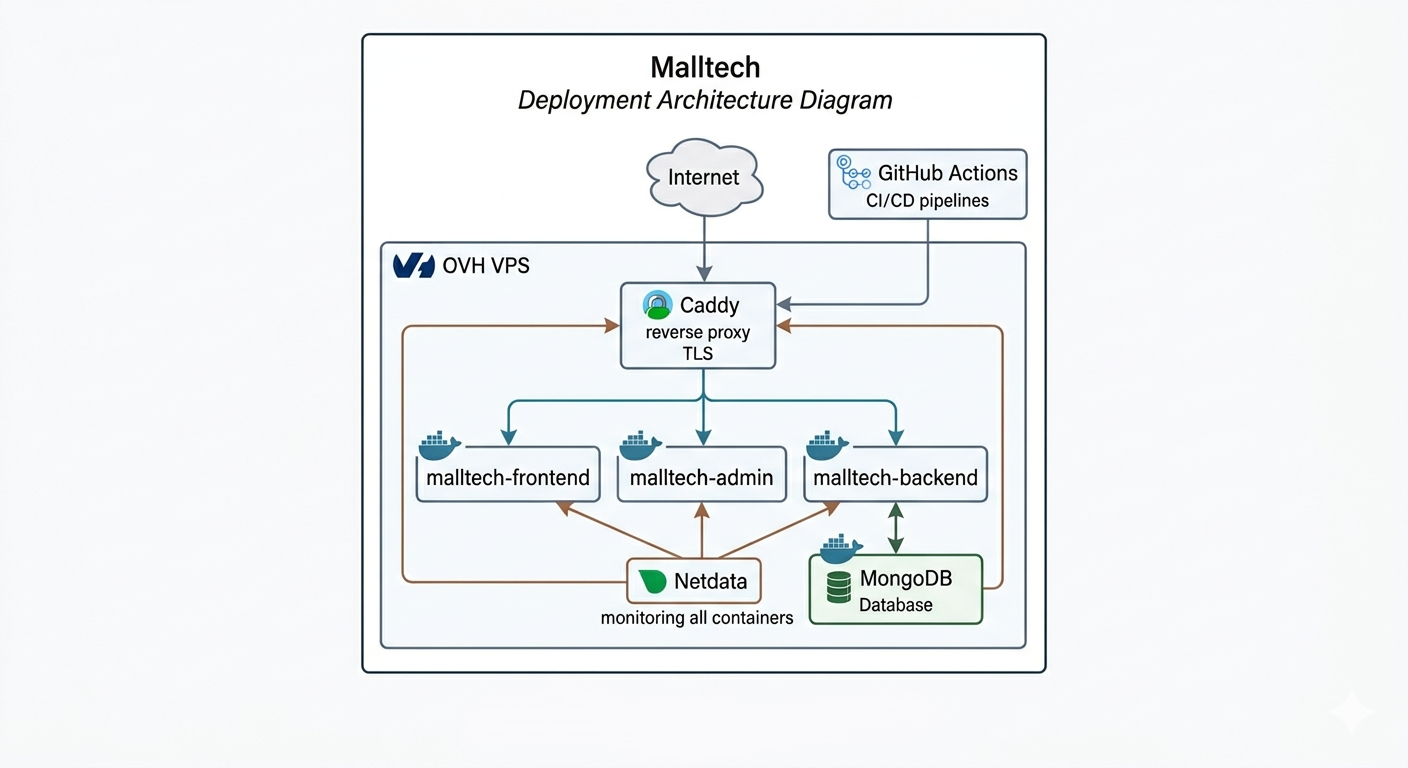
\includegraphics[width=\textwidth,height=0.45\textheight,keepaspectratio]{img/DeploymentArchitecture.png}
    \caption{Malltech deployment architecture}
    \label{fig:deployment}
\end{figure}

All containers share a \texttt{malltech} Docker bridge network. Only Caddy
exposes ports 80 and 443 to the host; all other services use internal Docker
networking exclusively.

\section{Backend Module Design}

The NestJS backend is organised into 15 feature modules, each encapsulating a
distinct business domain:

\begin{longtable}{|m{3.5cm}|m{10cm}|}
    \hline
    \textbf{Module}              & \textbf{Responsibilities}                                     \\
    \hline
    \endhead
    \endfoot
    \endlastfoot
    \hline
    \texttt{AuthModule}          & JWT strategy, session strategy, guards, password hashing      \\
    \hline
    \texttt{UsersModule}         & Customer CRUD, profile management                             \\
    \hline
    \texttt{CatalogModule}       & Categories, subcategories, brands, products, stock, 3D models \\
    \hline
    \texttt{BasketModule}        & Guest and authenticated basket operations                     \\
    \hline
    \texttt{OrdersModule}        & Order placement, status transitions, history                  \\
    \hline
    \texttt{PromotionsModule}    & Campaign management, automatic discount application           \\
    \hline
    \texttt{CouponsModule}       & Coupon CRUD, validation, usage tracking                       \\
    \hline
    \texttt{InvoicesModule}      & Sequential invoice numbering, PDF generation                  \\
    \hline
    \texttt{CreditNotesModule}   & Credit note issuance, PDF generation                          \\
    \hline
    \texttt{SupportModule}       & WebSocket gateway, ticket management, Discord bridge          \\
    \hline
    \texttt{NotificationsModule} & Email templates, SMTP dispatch                                \\
    \hline
    \texttt{CmsModule}           & Banners, blogs, authors, site configuration                   \\
    \hline
    \texttt{LocationsModule}     & Tunisian governorates, delivery fee configuration             \\
    \hline
    \texttt{SellingPointsModule} & Physical and digital store locations, cashier assignment      \\
    \hline
    \texttt{AnalyticsModule}     & Event recording, aggregate metrics                            \\
    \hline
    \caption{Backend NestJS modules}
    \label{tab:modules}
\end{longtable}

\section{Database Design}

MongoDB is used as the primary database. The following describes the key collections
and their relationships.

\subsection{Key Collections}

\begin{figure}[H]
    \centering
    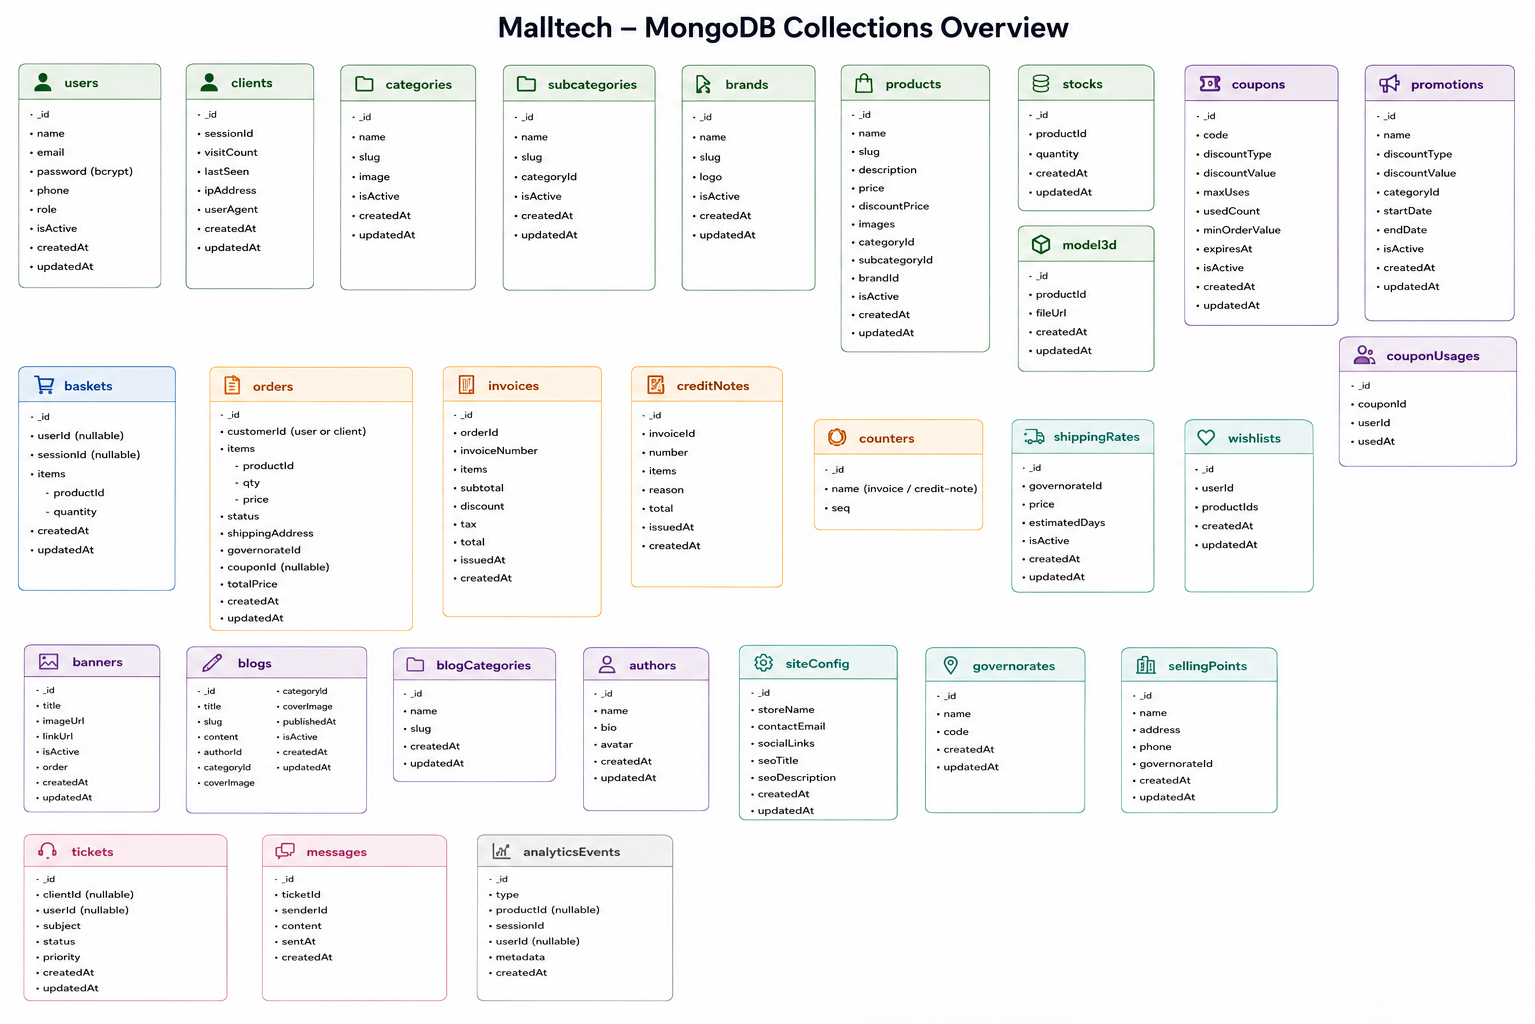
\includegraphics[width=\textwidth,height=0.45\textheight,keepaspectratio]{img/keycollection.png}
    \caption{Malltech database entity diagram}
    \label{fig:erd}
\end{figure}


\section{API Design}

\subsection{REST Conventions}

The API follows standard REST conventions:

\begin{itemize}
    \item Base URL: \texttt{https://api.domain.com}
    \item All routes are prefixed: \texttt{/auth}, \texttt{/products}, \texttt{/orders}, \texttt{/admin}, etc.
    \item JSON request/response bodies
    \item HTTP status codes: \texttt{200 OK}, \texttt{201 Created}, \texttt{400 Bad Request}, \texttt{401 Unauthorized}, \texttt{403 Forbidden}, \texttt{404 Not Found}, \texttt{409 Conflict}
    \item Pagination: query params \texttt{?page=1\&limit=20}, response includes \texttt{\{ data, total, page, totalPages \}}
\end{itemize}

\subsection{Key API Endpoints (Selected)}

\begin{longtable}{|m{1.5cm}|m{4.5cm}|m{2cm}|m{6cm}|}
    \hline
    \textbf{Method} & \textbf{Endpoint}                        & \textbf{Auth} & \textbf{Description}                  \\
    \hline
    \endhead
    \endfoot
    \endlastfoot
    \hline
    POST            & \texttt{/auth/register}                  & Public        & Register new customer                 \\
    \hline
    POST            & \texttt{/auth/login}                     & Public        & Login, returns JWT                    \\
    \hline
    GET             & \texttt{/products}                       & Public        & List products (filterable, paginated) \\
    \hline
    GET             & \texttt{/products/search}                & Public        & Full-text product search              \\
    \hline
    GET             & \texttt{/products/:slug}                 & Public        & Product detail                        \\
    \hline
    GET             & \texttt{/categories}                     & Public        & Category tree                         \\
    \hline
    POST            & \texttt{/basket/add}                     & Guest/Auth    & Add item to basket                    \\
    \hline
    GET             & \texttt{/basket}                         & Guest/Auth    & Get current basket                    \\
    \hline
    POST            & \texttt{/orders}                         & Auth          & Place order                           \\
    \hline
    GET             & \texttt{/orders/my}                      & Auth          & Customer's order history              \\
    \hline
    POST            & \texttt{/orders/:id/coupon}              & Auth          & Apply coupon to order                 \\
    \hline
    GET             & \texttt{/wishlist}                       & Auth          & Get wishlist                          \\
    \hline
    POST            & \texttt{/wishlist/:productId}            & Auth          & Toggle wishlist item                  \\
    \hline
    GET             & \texttt{/governorates}                   & Public        & List governorates                     \\
    \hline
    GET             & \texttt{/blogs}                          & Public        & Blog article listing                  \\
    \hline
    POST            & \texttt{/support/tickets}                & Guest/Auth    & Open support ticket                   \\
    \hline
    GET             & \texttt{/admin/orders}                   & Admin         & All orders, filterable                \\
    \hline
    PATCH           & \texttt{/admin/orders/:id/status}        & Admin         & Update order status                   \\
    \hline
    POST            & \texttt{/admin/invoices/:id/pdf}         & Admin         & Generate invoice PDF                  \\
    \hline
    POST            & \texttt{/admin/invoices/:id/credit-note} & Admin         & Issue credit note                     \\
    \hline
    GET             & \texttt{/admin/analytics/events}         & Admin         & Analytics event data                  \\
    \hline
    \caption{Key API Endpoints}
    \label{tab:api_endpoints}
\end{longtable}

\subsection{WebSocket — Support Gateway}

The support module exposes a Socket.IO namespace for real-time messaging:

\begin{longtable}{|m{3.5cm}|m{3cm}|m{7.5cm}|}
    \hline
    \textbf{Event}                  & \textbf{Direction}          & \textbf{Payload}                 \\
    \hline
    \endhead
    \endfoot
    \endlastfoot
    \hline
    \texttt{join\_ticket}           & Client $\rightarrow$ Server & \texttt{\{ ticketId \}}          \\
    \hline
    \texttt{send\_message}          & Client $\rightarrow$ Server & \texttt{\{ ticketId, content \}} \\
    \hline
    \texttt{new\_message}           & Server $\rightarrow$ Client & \texttt{\{ ticketId, message \}} \\
    \hline
    \texttt{ticket\_status\_update} & Server $\rightarrow$ Client & \texttt{\{ ticketId, status \}}  \\
    \hline
    \caption{WebSocket Events for Support}
    \label{tab:ws_events}
\end{longtable}

\section{Sequence Diagrams}

\subsection{Product Search Flow}

\begin{figure}[H]
    \centering
    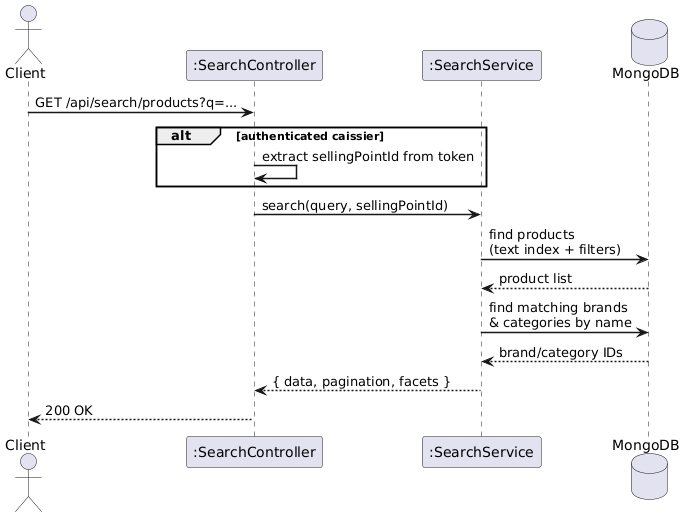
\includegraphics[width=\textwidth,height=0.45\textheight,keepaspectratio]{img/searchSeqDiagram.png}
    \caption{Product search sequence}
    \label{fig:seq_search}
\end{figure}

\subsection{Order Placement Flow}

\begin{figure}[H]
    \centering
    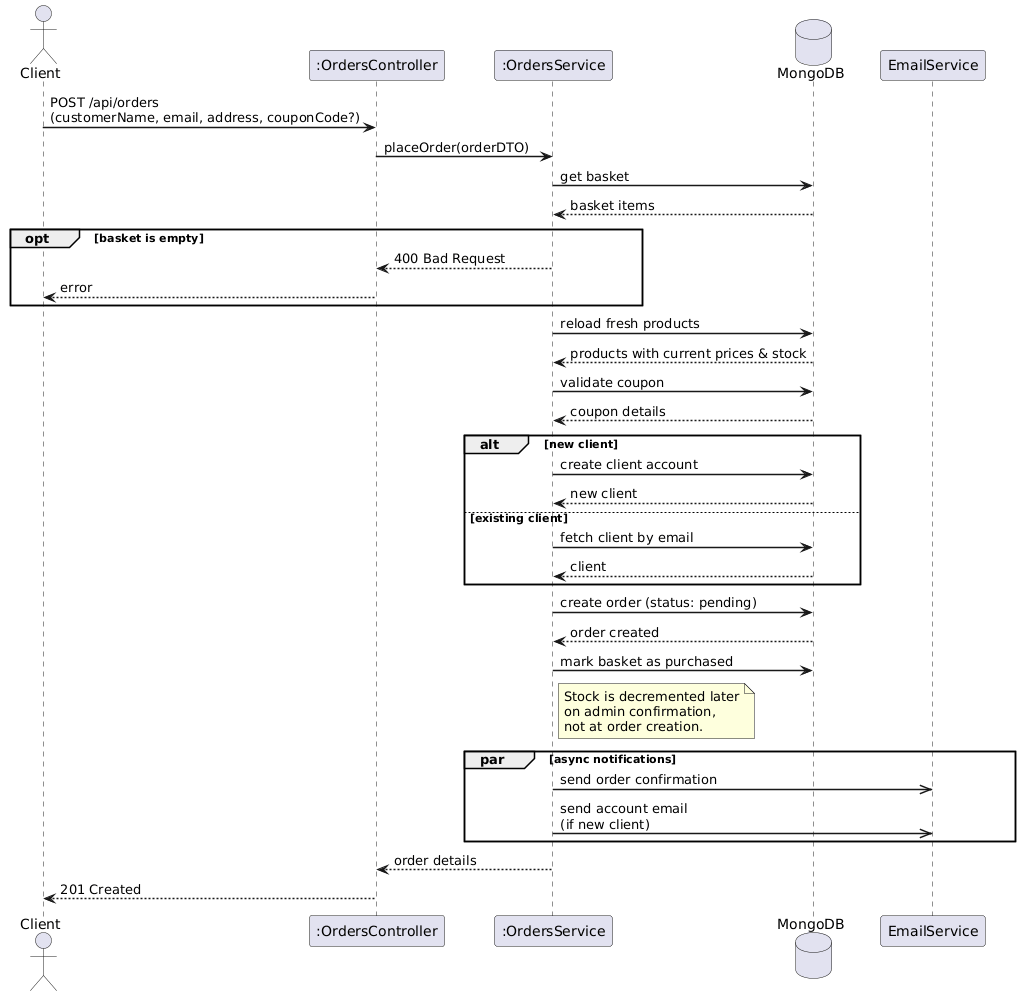
\includegraphics[width=\textwidth,height=0.45\textheight,keepaspectratio]{img/orderSeqDigram.png}
    \caption{Order placement sequence}
    \label{fig:order_flow}
\end{figure}

\section*{Conclusion}
This chapter presented the three-service architecture, the NestJS module decomposition,
the MongoDB data model, and the REST API design. The following chapter covers the
concrete implementation of these designs.
